\Chapter{DISCUSSION}\label{sec:Theme3}

\section{Interprétation des résultats}
Les résultats obtenus ont permis d’atteindre en tout ou en partie l’ensemble des sous-objectifs énoncés dans le chapitre~\ref{chapitre_methode}.%, voir Tableau~\ref{tab:synthese_travaux}.

\paragraph{SO-1 Accomplissements}
Simplification de l’écriture de technique dans le générateur de code avec l’utilisation de «f-string», de la bibliothèque «Code-writer» et de la bibliothèque «lxml».\\
Ajout de «Wizard» pour configurer le MVC selon des paramètres.\\
Amélioration de l’importation des bases de données externes.\\
Support de la génération de code par des données.\\
Augmentation de technique de génération de code, support des templates «Qweb», ajout du type de données géospatiale.

\paragraph{SO-1 Feuille de route}
Implémenter les fonctionnalités manquantes dans la GUI pour générer les MVC d’un module.\\
Augmenter le nombre de technologies à supporter l'importation des données.\\
Ajouter le support de génération sur différentes architectures.\\
Il manque des techniques de sécurité à personnaliser, comme l’anonymisation des données.\\
Générer automatiquement une documentation sur l’utilisation d’une technique. \\
Supporter la génération sur d’autres systèmes ERP libres tel que Tryton\footnote{\url{https://www.tryton.org}}.

\paragraph{SO-2 Accomplissements}
Extraction du code via l’utilisation d’un AST et extraction des méta-données dans les fichiers XML.\\
Amélioration continue sur la génération de code grâce à la reproduction à l’aide de l’extraction du code.\\
Un outil pour aider à la création de technique de génération à l’aide d’un générateur de générateur de code.\\
Le générateur de code est accompagné de tests de validation en reproduisant l’ensemble des techniques en démonstration.\\
La génération de code applique des règles de codage standardisées.

\paragraph{SO-2 Feuille de route}
Finaliser l’implémentation de l'auto génération sur l’automate.\\
Mise à jour des tests pour atteindre une couverture de code à 100\%.\\
Ajout de test sur les techniques d’extractions de code tel que le PHP.

\paragraph{SO-3 Accomplissements}
Ajout de nouvelles techniques et une classification de ceux-ci.\\
Rendre accessible une interface graphique pour paramétrer la génération de code.\\
Rendre accessible une interface de programmation pour utiliser toutes les fonctionnalités de l’automate.

\paragraph{SO-3 Feuille de route}
Ajout de paramètres pour faire plus de personnalisation sur les techniques et les séparer une par module.\\
Supporter les fonctionnalités manquantes sur toutes les techniques pour l’interface graphique.\\
Support l’accès à la création de méta-données par la rétro-ingénierie via l’interface graphique.

\paragraph{SO-4 Accomplissements}
Intégration dans un système de distribution via un Docker.

\paragraph{SO-4 Feuille de route}
Développer une synchronisation entre les instances pour permettre de la redondance.\\
Développer une gestion de son infrastructure via le générateur de code.\\
Faire participer l’automate à la maintenance de l’infrastructure de déploiement.\\
Utiliser d’autres systèmes de conteneur en distribution qui sont libres comme «Pod»~\footnote{\url{https://podman.io/}}.\\
L’automate doit avoir la capacité de valider techniquement si le logiciel est AGPLv3 au moment de l’exécution

\paragraph{SO-5 Accomplissements}
Test de la génération sur un module existant de la communauté nommé «auto\_backup».\\
Des modules de gestion de projet ont été générés pour faire le suivi de la conception fonctionnelle et de l’amélioration continue.\\
Le projet Accorderie a bénéficié du générateur de code pour la migration de la base de données vers Odoo.\\
Le projet Portail CEPPP a bénéficié du générateur de code pour la migration du code PHP vers Odoo, ainsi que de l’aide au développement de la section Portail.

\paragraph{SO-5 Feuille de route}
L’automate doit supporter la demande de «Pull Request» sur les projets Git respectif lorsqu’il y a une amélioration. Il doit faire le suivi et s’assurer de suivre les règles de contributions de la communauté.\\
Développer d’autres modules de gestion de projet pour l’accompagnement dans le développement de projet client.\\
Développer des modules de gestion de communauté sur des projets logiciels libres.\\
Développer le suivi du développement des modules communautaires avec une traçabilité sur les résultats avec des métriques de génie logiciel.

\subsection{Comment les résultats obtenus soutiennent le libre}

Le réseau d’entraide a besoin d’un support technologie libre, puisque permettre aux participants de respecter leur 4 libertés vont permettre de pouvoir s’adapter à des situations d’urgence et apporter des solutions rapidement.

\paragraph{Étudier}
La rétro-ingénierie a permis à l’automate de comprendre certaines fonctionnalités pour pouvoir recréer les méta-données adéquatement pour la reproduction.

\paragraph{Copier}
L’auto-générateur a été mis en place, il reste à auto-reproduire l’automate par son module principale de générateur de code.

\paragraph{Modifier}
Rend accessible la rétro-ingénierie tout en exécutant des mises en forme de code et validation de qualité logiciel.

\paragraph{Utiliser}
L’automate a la capacité d’utiliser ses fonctionnalités générées et d’exécuter des scripts d’automatisation à des périodes de temps adaptable.

\subsection{Couverture des tests}

Les tests devraient couvrir 100\% du code, cependant la couverture est de 84\% pour 3 raisons :

\begin{enumerate}
    \item Il y a du code fonctionnel non testé, il manque des tests;
    \item Il y a du code désuet qu’il faut nettoyer ou refactoriser;
    \item La gestion des erreurs n’est pas couverte, il faudrait les ignorer dans le test de couverture et faire des tests unitaires qui valide la gestion des erreurs.
\end{enumerate}

\subsection{Projet Accorderie}
La migration de la base de données a été réussie, mais elle est encore à ce jour en adaptation vers un modèle Odoo plus intégré au ERP. Les efforts ont été mis pour la création d’une interface utilisateur avec des technologies qui n’étaient pas à la base supportées dans Odoo.

\subsection{Projet Portail CEPPP}

La signification que le nombre de lignes de XML aurait diminué, c’est que l’automate génère de base toutes les vues de tous les champs. Au moment de la ré-ingénierie, il y a eu beaucoup de nettoyage et de données XML effacées. Cependant, le développeur va mettre plus de code Python pour développer des logiques qui ne sont pas supportés par l’automate. Le Javascript ajouté sert à supporter les dates dans le portail. L’ajout de CSV sert pour l’ajout de permissions et rôles pour l’anonymisation.

Après la première migration par l’extraction du modèle de données par PHP, le client a pu testé la plateforme pour avoir une idée à quoi ressemblerait l’utilisation dans l’espace administration de leur modèle de données et ils ont fait des demandes de changement. Une analyse a été effectuée, nous avons utilisé le générateur de code pour générer les vues portails et fait une ré-ingénierie manuelle du modèle et des vues pour obtenir le résultat désiré. Une des fonctionnalités implémentés est l’anonymisation des données pour certains groupes d’utilisateurs, pour pouvoir visualiser des données sans avoir d’information personnelle sur le patient.

\subsection{Avancement de la technopoïèse}

Avec la figure~\ref{fig:dia_auto_machine_discussion}, la ré-ingénierie manuelle est le processus habituel d'un développeur. Avec ce projet, nous avons une autopoïèse fonctionnelle semi-automatique, avec intervention humaine, puis une allopoïèse complète avec intervention humaine lorsque est en dehors des techniques maîtrisés par le robot codeur. Le développement est au centre d'un réseau d'entraide avec des guides pour gérer son projet technologique.

\subsection{Réalisation du robot générateur de code}

Dans la revue littérature section~\ref{robot_logiciel_developpeur_revue}, nous avons déterminé 4 critères pour définir un robot codeur :
\paragraph{Autonomie}
Nous avons des résultats qui démontrent 100\% d'autonomie dans quelques contextes, voir les résultats sur les tests de validation section~\ref{test_validation_generation_code_resultat}. Cependant, le robot codeur n'est pas 100\% autonome pour tous les contextes, il a besoin d'intervention humaine pour des personnalisations ou des techniques non supportés.

% TODO une fois qu'on aura supporté plus de technique et l'autopoïèse entière, la prochaine étape serait de le faire fonctionner en continue. Bien qu'il soit capable via l'interface graphique, les efforts n'ont pas été effectué pour cette capacité.

\paragraph{Adaptable}
Le robot codeur est adaptable, il génère 6 composantes, voir résultat d'architecture section~\ref{architecture_result} : web, website, portail, snippet, migration de données entrants et migration de modèle de données entrants. De plus, il est capable d'interagir avec des technologies en dehors d'Odoo telles que d'extraire du code externe en PHP du logiciel SuiteCRM et des bases de données externes (MySQL/SQL Server/PostgreSQL) pour importer des modèles de données et migrer des données.

% TODO il faudrait supporter la génération de technologies externes, nous travaillons présentement à générer des applications mobiles natives, ou même générer des modules sur d'autres plateforme ERP tel que Tryton ou NextERP.

\paragraph{Compétences techniques}
Le robot codeur contient plusieurs compétences techniques qui sont décrites dans les résultats section~\ref{result_technique_developpe}. De plus, il permet la personnalisation pour chacune des composantes du nombre de champs, des types de champs et du type d'affichage associé aux champs.

% TODO les techniques ont été développés comme preuve de concept, il manque de mâturité et de personnalisation. 

\paragraph{Compétences socials}
Le robot codeur donne accès à des outils pour le développeur. Il y a un interface graphique LCNC qui permet la paramétrisation pour la génération de code. Il y a aussi un interface de code pour paramétrer le fonctionnement de la génération accompagné de la rétro-ingénierie et il permet d'accompagner le développeur dans l'évolution de son module. Il contient aussi une fonctionnalité pour afficher les différences de code, créer des statistiques sur les lignes de codes, montrer la couverture de code, etc.

% TODO manque l'outil en temps réel, ce n'est pas supporté dans Odoo, il faut utiliser une application tierce tel que Etherpad et ajouter les méthodes de synchronisation des mises à jour sur les données. Il manque l'accès directe aux script à la racine du projet ERPLibre pour contrôler les outils de contrôle de la qualité. Collaboration, conscience professionnelle, résolutions de problèmes en équipe, communication efficace, adaptivité sur les livrables et exigences clientes

\begin{figure}
\centering
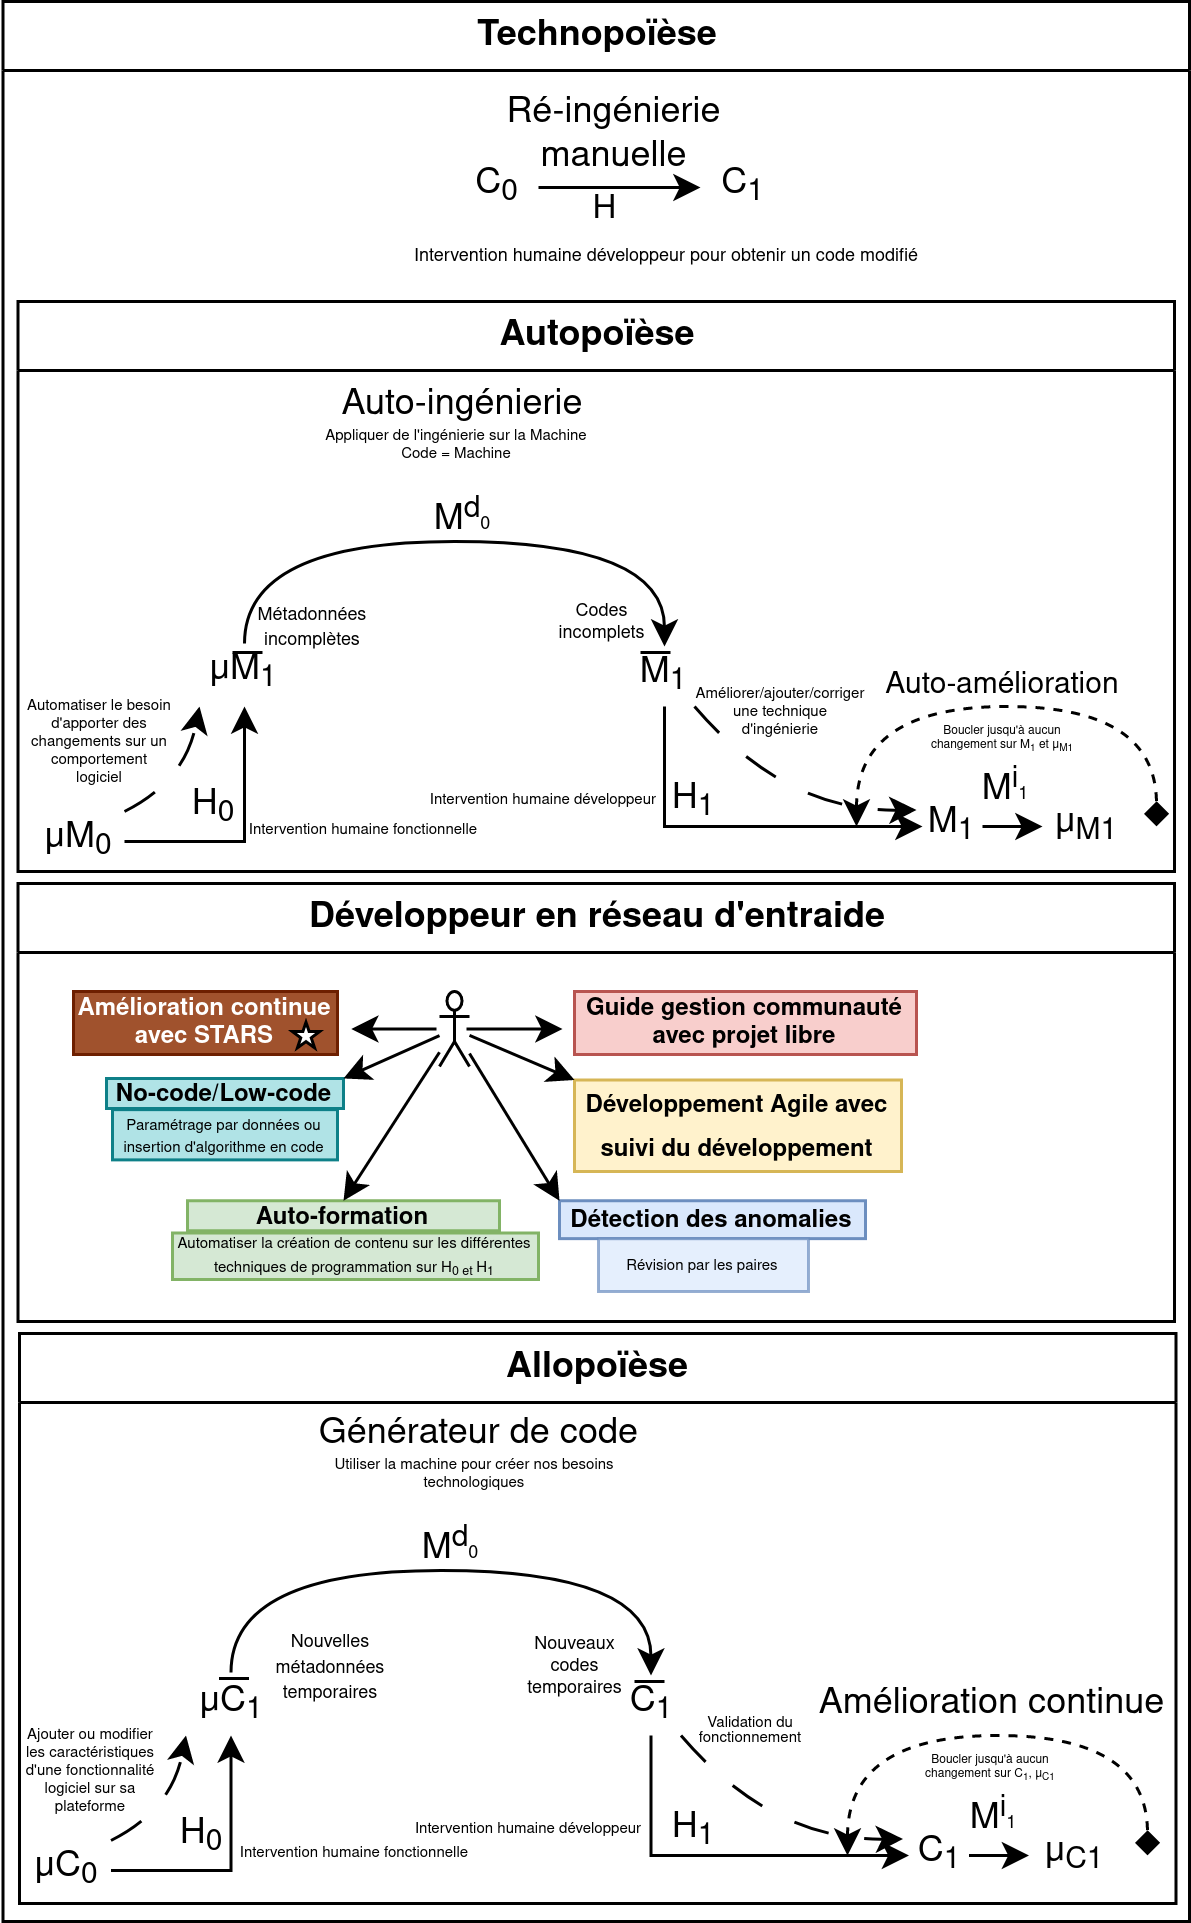
\includegraphics[height=8.5in]{images/auto_machine_discussion.drawio.png}
\caption{Architecture de l'automate}
\label{fig:dia_auto_machine_discussion}
\end{figure}

\section{Forces et limitations}
% TODO dire en quoi ce que tu as fait améliore l’état de l’art décrit dans la littérature
% TODO décrire les limitations/faiblesses de ce que tu as produit comme logiciel/résultats

\subsection{Génération par gabarit}

L’utilisation de f-string et de la bibliothèque Code-writer permet de faciliter la lecture du développeur puisque le code du générateur se rapproche plus du résultat généré.

\subsection{Template de «A template-based code generator for web applications»}
Cette application n’est pas accessible facilement au public, il sera difficile de comparer l’efficacité du côté pratique. Ce qui peut être comparé, c’est les performances, hors ça n’a pas été testé dans notre travail, puis l’architecture, mais le fait qu’il n’utilise pas ORM explique la différence d’architecture. Sinon il n’utilise pas de rétro-ingénierie et son générateur n’est pas adapté sur une communauté existante.

\section{Avenues futures d’amélioration ou d’utilisation}
% TODO dire ce qui doit être fait pour que les aspects d’utilisabilité de ton logiciel en terme de communauté, de libre, etc soient complets.

\subsection{Support de développement de module dans la communauté Odoo}

ERPLibre supporte Odoo 12, puisque c’est lui qui supporte le plus de modules. Cependant, ces données représentent seulement ceux des repos utilisés par ERPLibre, il y a en beaucoup plus dans la communauté. C’est pourquoi il faut faire une recherche de ces modules dans la communauté et entreprises, et les rendre accessible par une base de données publiques~\footnote{Comme fait sur \url{https://odoo-code-search.com/}}.

Selon l’évolution, il faudrait migrer vers la version 14.0 en 2024. Donc il faut falloir supporter la migration de modules vers des versions supérieures.

\subsection{Amélioration du générateur code}

Il faut intégrer la génération de code à l’intérieur des instances clientes dans l’objectif qu’ils soient accessibles de son gestionnaire de déploiement pour y ajouter les nouvelles fonctionnalités, démarrer la mise à jour, les tests, les améliorations, la migration, importation. Les instances clientes devraient proposer aux clients via les interfaces 

% Intégration de plusieurs types de réseaux de neurones accessibles librement, il doit être compatible avec le libre.

% Il faut suggérer aux clients des améliorations et de communiquer avec leurs gestionnaires de déploiements.

% Un générateur de code a été créé. L’embryon est créé, il faut terminer sa génération du générateur de code. Les déviances sont déjà créées

Une fois que le générateur de code aura atteint 100\% d’auto-génération, il restera limité à produire que les fonctionnalités qu’il utilise. Donc s’auto-générer fait office de test. Il faut faire des tests pour les fonctionnalités qu’il n’utilise pas (ou les combinaisons non utilisés) pour se reproduire. Il reste à auto-générer toutes ses techniques dans des modules qui font de l'héritage sur le générateur de code.

% Ajout de la génération de test de base, génération de documentation, mise à jour, migration lors d’une mise à jour sur les données, migration d’une mise à jour de la plateforme.

\subsubsection{Amélioration de l’architecture}
Parallélisation de tout le code tout le temps lorsque possible.

Automatisation de la configuration pour le déverminage, automatiser la détection des anomalies, améliorer l’interface no-code pour pouvoir accomplir les mêmes étapes que le mode de paramétrisation «Code hook». Supporter de nouvelles architectures dans la génération de code comme des applications Cordova pour le support mobile natif, des extensions Javascript dans Gnome Shell pour étendre les fonctionnalités du ERP directement sur le bureau d’un ordinateur sans passer par un navigateur web, générer des scripts de développement dans le projet ERPLibre qui ne dépendant pas d’Odoo, ou même supporter des applications embarqués.

De plus, il serait pertinent de supporter d’autres ERP externe comme NextERP ou Tryton qui sont des solutions libres. Cela va permettre la migration entre ERP des fonctionnalités et encourager l’utilisateur à prendre une solution entièrement AGPLv3 avec une communauté qui le supporte dans cette philosophie.

Problème d’extraction, il était dans le générateur de code au départ dans le développement, il y a donc une extraction à deux endroits qui rend complexe la gestion du code. Au fil de la progression du développement, l’extraction de données par rétro-ingénierie s’avère plus efficace que les méta-données du module dans le système Odoo.

L’auto-ingénierie sur la machine est en cours d’exécution sur le module de base, il faudrait aussi supporter les modules hérités qui sont définis comme des techniques.

Découper les fonctionnalités d'extraction et de génération, puis les séparer dans des modules des techniques du générateur de code.

Il faudrait réduire le nombre de technique dans Base pour qu’ils soient des modules externes par technique, ça faciliterait le changement d’architecture sur la gestion des méta-données, à adapter selon la rétro/ré-ingénierie.

% TODO mettre photo d'amélioration architecture

Les travaux d’amélioration devront être effectués après l’auto-génération.

\subsubsection{Amélioration de la gestion de projet et statistiques}

Le générateur de code doit offrir des outils de gestionnaire de projet pour suivre le développement, faire la liaison entre les demandes clients et les avancements des développeurs.

De plus, puisque l’état des méta-données évoluent, il devient difficile de faire le suivi des performances du générateur de code, puisqu’il vient aider dans les boucles d’itérations qui ne nécessitent pas de faire des commits, puisqu’on commit lorsque le tout est stable. Ainsi il faudrait faire des statistiques sur ces itérations pour évaluer la contribution du générateur.

Il manque l’analyse des différences de code sur les différentes sections générées.

\subsubsection{Suite du développement du générateur de code}

Il faudrait qu’il génère des tests fonctionnels, de la documentation fonctionnelle et développe la migration de données selon les changements des versions antérieurs. Un suivi des fonctionnalités selon les exigences clientes.

Une fois l’architecture mise à jour, la prochaine étape est de tester sa mise à niveau de tous les modules dans la communauté et détecter les techniques manquantes par supervision du développeur pour les implémenter. Une fois qu’il aura géré tous les modules de la communauté, on pourra implémenter la migration vers des mises à jour de la plateforme, c’est-à-dire vers Odoo 14, puis vers Odoo 16.

Une fois que l’auto-poïèse sera en place sur la gestion de la machine, la prochaine étape sera de faire l’auto-poïèse sur tout le code Odoo pour le développement de l’architecture.

\subsection{Projet Accorderie}
Maintenant qu’une plateforme sur le site web a été développée, il faudrait poursuivre la mise à jour du générateur de code pour supporter ce type de plateforme pour des projets futurs similaires.

\subsection{Projet Portail CEPPP}
Le générateur de code a été utilisé en début de projet et à fait économiser du temps de développement et réduit les erreurs possibles de retranscription du langage PHP au langage Python, ainsi que la génération des vues admin et portail. Cependant, l’automate a arrêté d’être utilisé au moment qu’on a commencé à diverger vers des fonctionnalités personnalisées qu’il ne pouvait pas supporter. Il faudra supporter ces fonctionnalités pour les futurs projets.

% \subsection{Déploiement - distribution}
% TODO, que c’est un sous-objectif supplémentaire qui n’a pas été touché.

\subsection{NLP}
La technologie NLP va permettre de comprendre des textes rédigés par l’utilisateur et l’associer à des techniques de programmation.

% TODO Définir le besoin 
% TODO parler d’émotion et empathie

% Qu’est-ce qu’il faudrait développer pour se rendre au stade automate codeur?

Le NLP est une solution alternative pour interfacer avec l’utilisateur et communiquer avec pour développer des logiciels.

Suggestion d’explorer l’outil libre : Utiliser «HuggingFace» qui contient une grande communauté autour du développement d’un réseau de neurones pour faire du NLP par exemple, c’est compatible avec le logiciel libre.

% \subsection{DevOps}
% Il faudrait mettre en place les outils de dev ops.
% Mise à jour des bibliothèques (avoir une vue d’ensemble autre que Poetry)

% \subsection{Gestion de communauté}
% Un downtime de plus d’une journée cause drastiquement un abandon des participants à l’utilisation d’une technologie au sein d’une autre.

\subsection{Réseau d’entraide}

Il doit y avoir un responsable pour chaque localité accompagné de l’automate pour répondre à ses besoins de numérisations via une souveraineté numérique. C’est le gestionnaire de communauté.

Chaque projet d’urgence doit être capable d’avoir une équipe en charge pour accélérer la résolution de problèmes locaux.

% \subsection{Technopoïèse}
% À titre de discussion sur la signification de technopoïèse.

% Auto-répliqueur : une machine qui se copie lui même.
% Allopoïèse : une machine qui crée une autre machine avec des éléments extérieurs, l’inverse de l’autopoïèse.
% Autopoïèse : la propriété d’un système de se produire lui-même, en permanence et en intéraction avec son environnement, et ainsi de maintenir son organisation (structure) malgré son changement de composants (matériaux) et d’informations (données).
% REF https://fr.wikipedia.org/wiki/Autopo%C3%AF%C3%A8se
% Technopoïèse : une technologie qui a la propriété de se produire lui-même …
% «Une technologie pour étudier la vie humaine, des nouvelles sociétés et les accompagner dans leur développement d’autopoïèse. »
% La technopoïèse doit être développée dans un contexte de logiciel libre pour mettre au centre le réseau d’entraide et avoir le contrôle sur les dérives non éthiques.
% Outil passif utilisé par les humains pour jouer un rôle actif dans la création de la société et de la culture en façonnant leur environnement et leur mode de vie. Comprendre comment les technologies influencent la façon dont les individus interagissent et comment elles peuvent être utilisées pour améliorer la vie des gens, de manière responsable et éthique.

% \subsection{Robot codeur libre}

% Les robots codeurs peuvent être programmés pour effectuer différentes tâches, telles que la génération de code source, la correction de bugs, l'optimisation des performances, la maintenance des systèmes et la gestion de versions. Certains robots codeurs peuvent même apprendre à partir d'exemples de code existant et développer des algorithmes en se basant sur des données d'entrée.

% Les robots codeurs peuvent également améliorer la qualité du code en réduisant les erreurs humaines, en accélérant les tests et en appliquant des pratiques de codage cohérentes.»

% TODO projet d’impression 3D à distance, avec des propriétaires de machines qui les entretiennent.

% TODO connaissance de la physique et les appliquer, optimisation pour accompagner les communautés dans leur gestion d’urgence
% TODO doit reproduire les 4 libertés pour l’utilisation, l’accompagner dans son développement pour améliorer ses habitudes de vies par lui même sans dépendre d’autrui, restons en communauté locale pour réduire la consommation.
% TODO faciliter l’intégration de l’intération entre notre robot personnel et celui d’une technologie externe.
